

%aca va el ejercicio

Se implementaron dos compuertas NOT con tecnología BJT: una variante con un transistor NPN (BC337) y otra con un transistor PNP (BC557). Sus diseños se pueden observar en la siguiente figura.


\begin{figure}[H]
  \centering
    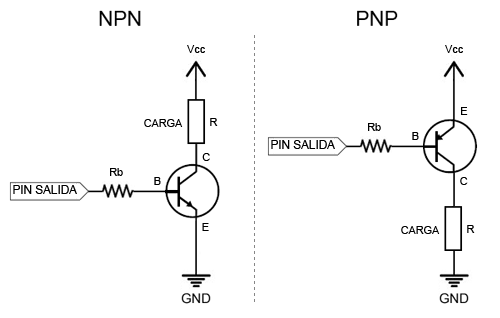
\includegraphics[width=0.5\textwidth]{ejercicio1/circuitos.png}
    \caption{Circuitos inversores para transistores NPN y PNP.}
\end{figure}

Midiendo con un osciloscopio la entrada y la salida del circuito y haciendo uso del modo XY, se obtuvo la curva caracter\'istica de tensi\'on de cada compuerta.

A partir de estas curvas, se obtuvieron los niveles de voltaje de input y output para los niveles altos y bajos de ambas compuertas, as\'i como los m\'argenes de ruido. Estos figuran en la siguiente tabla.
\begin{center}
\begin{table}[H]
\begin{tabular}{|l|l|l|}
\hline
                          & NPN   & PNP    \\
High Level Input Voltage  & 1.18V & 4.28V  \\
Low Level Input Voltage   & 518mV & 3.08V  \\
High Level Output Voltage & 4.88V & 4.53V  \\
Low Level Output Voltage  & 462mV & 12.5mV \\
High Noise Margin         & 3.7V  & 0.25V  \\
Low Noise Margin          & 56mV  & 3.067V
\end{tabular}
\end{table}
\end{center}
Posteriormente, midiendo las curvas de entrada y salida en simult\'aneo, se obtuvieron los tiempos de transición y las demoras de propagación para ambas compuertas. Luego, se cargaron las compuertas con un capacitor de 10nF, y obteniendo la derivada de la tensión de salida, utilizando la ley de Ohm para capacitores pudo determinarse la corriente m\'axima a trav\'es de la compuerta. Estos datos figuran en la siguiente tabla.
\begin{center}
\begin{table}[H]
\begin{tabular}{|l|l|l|}
\hline
                                       & \textbf{NPN} & \textbf{PNP} \\ \hline
\textbf{Propagation Delay High to Low} & 270 ns       & 860 ns       \\ \hline
\textbf{Propagation Delay Low to High} & 3.22 $\mu s$      & 101 ns       \\ \hline
\textbf{Transition Time High to Low}   & 230 ns       & 538 ns       \\ \hline
\textbf{Transition Time Low to High}   & 840 ns       & 159 ns       \\ \hline
\textbf{Max Output Current}            & 14.68mA      & 9.25mA       \\ \hline
\end{tabular}
\end{table}
\end{center}

\subsubsection{Mediciones en osciloscopio}
\begin{multicols}{2}

\begin{figure}[H]
  \centering
    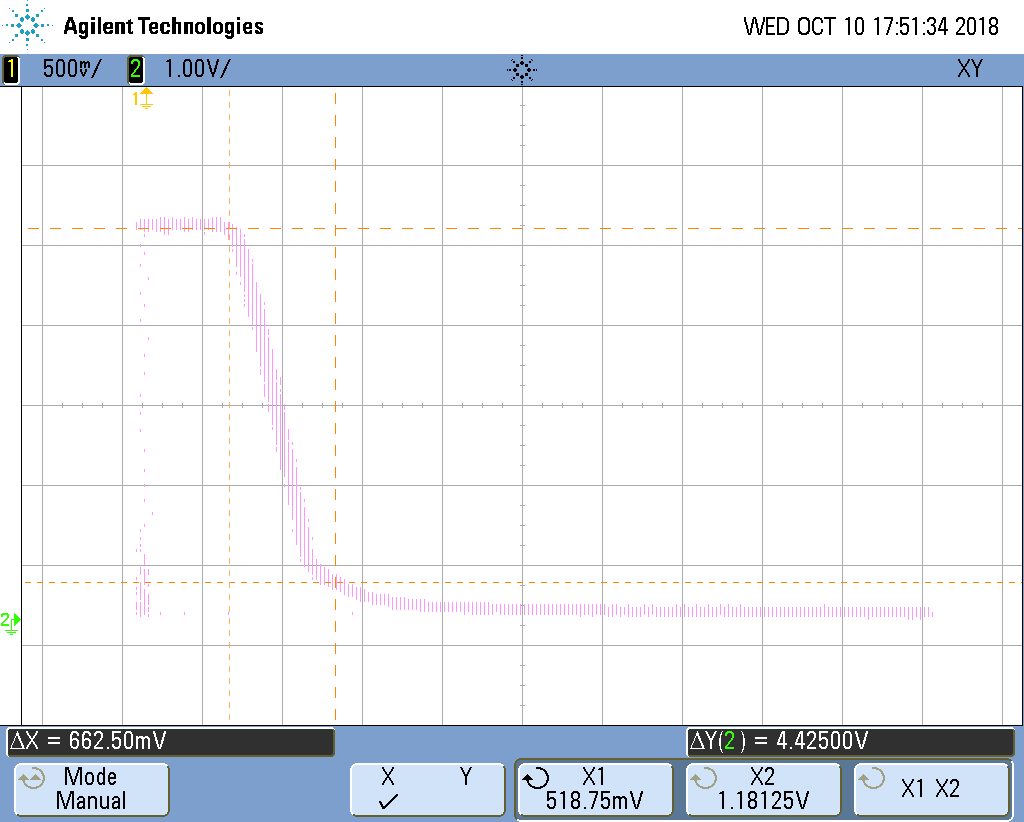
\includegraphics[width=0.4\textwidth]{ejercicio1/scope_x_Punto1_NPN}
    \caption{Curva caracter\'istica NPN: datos de input.} %caption abajo
\end{figure}

\begin{figure}[H]
  \centering
    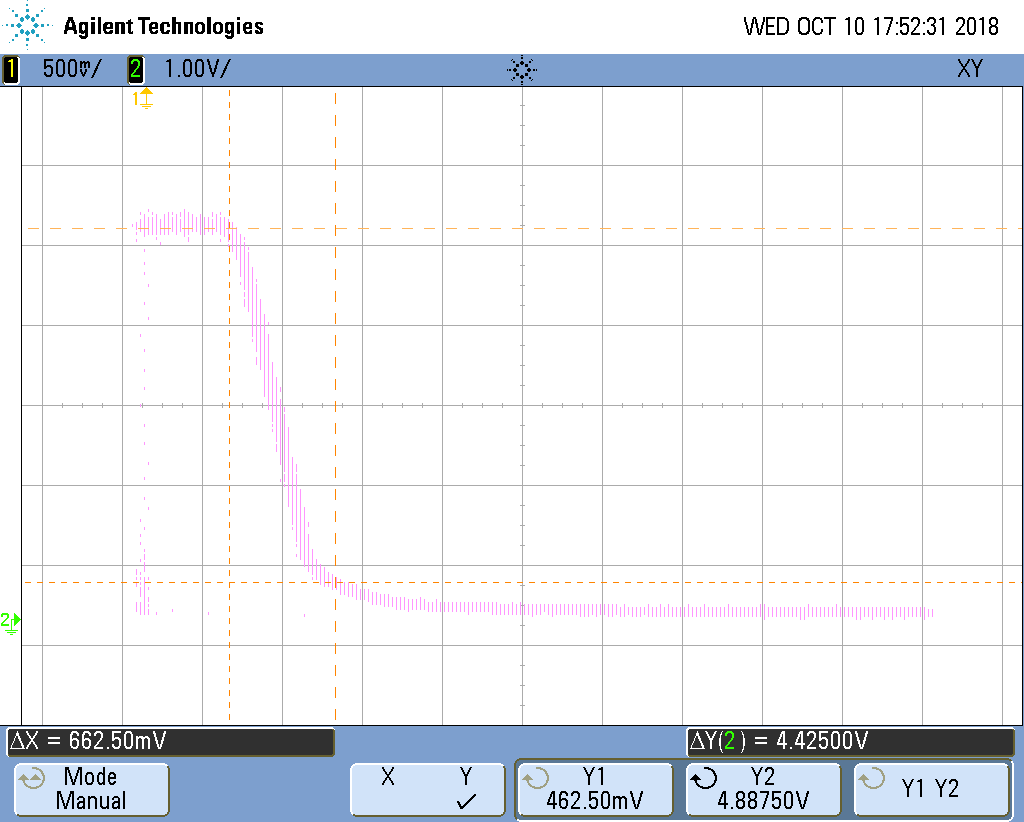
\includegraphics[width=0.4\textwidth]{ejercicio1/scope_y_Punto1_NPN}
    \caption{Curva caracter\'istica NPN: datos de output.} %caption abajo
\end{figure}

\begin{figure}[H]
  \centering
    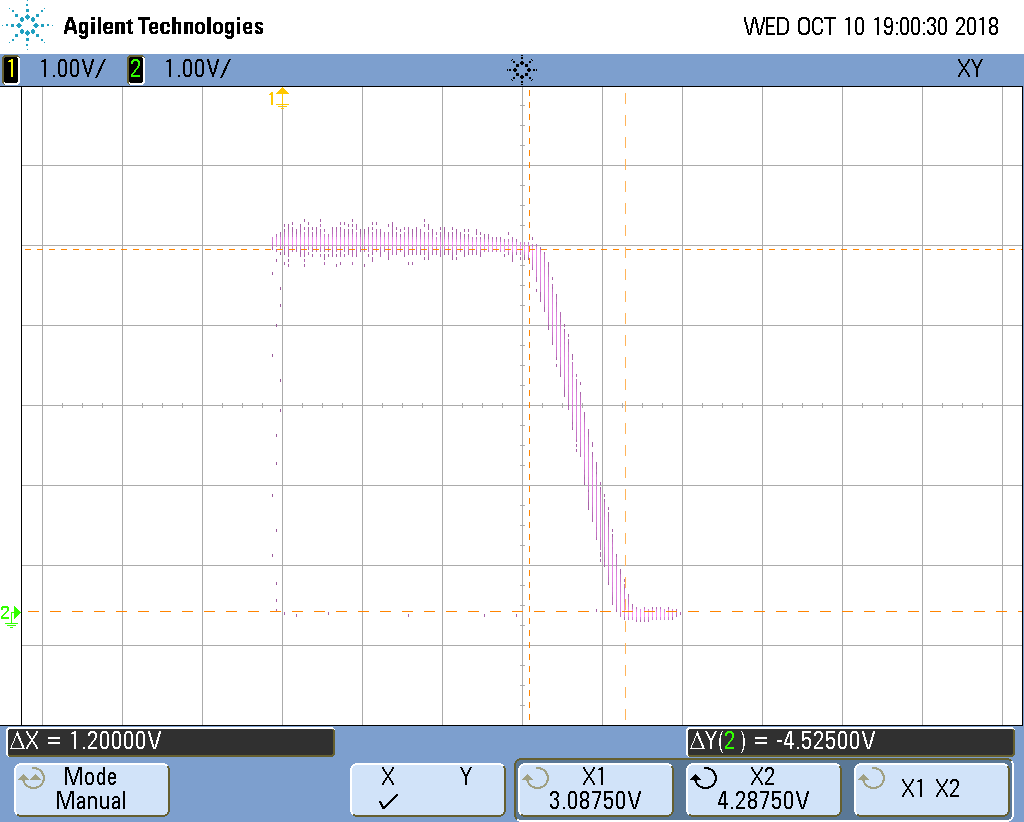
\includegraphics[width=0.4\textwidth]{ejercicio1/scope_x_Punto1_PNP}
    \caption{Curva caracter\'istica PNP: datos de input.} %caption abajo
\end{figure}

\begin{figure}[H]
  \centering
    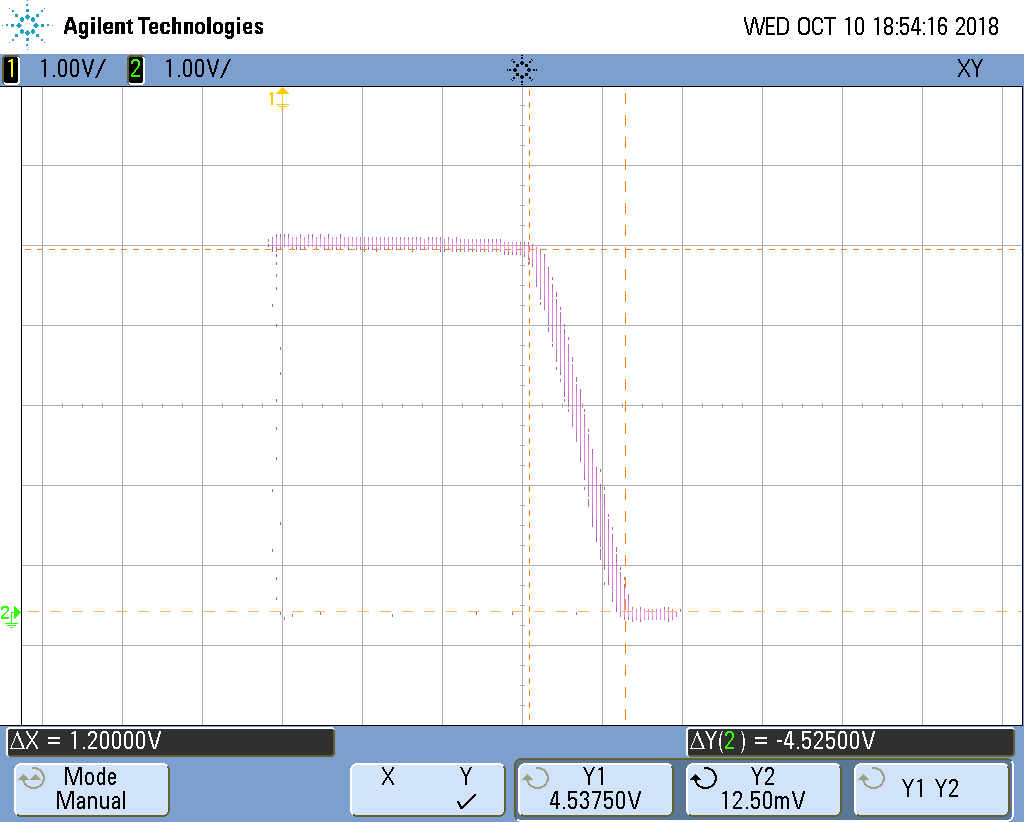
\includegraphics[width=0.4\textwidth]{ejercicio1/scope_y_Punto1_PNP}
    \caption{Curva caracter\'istica PNP: datos de output.} %caption abajo
\end{figure}

\begin{figure}[H]
  \centering
    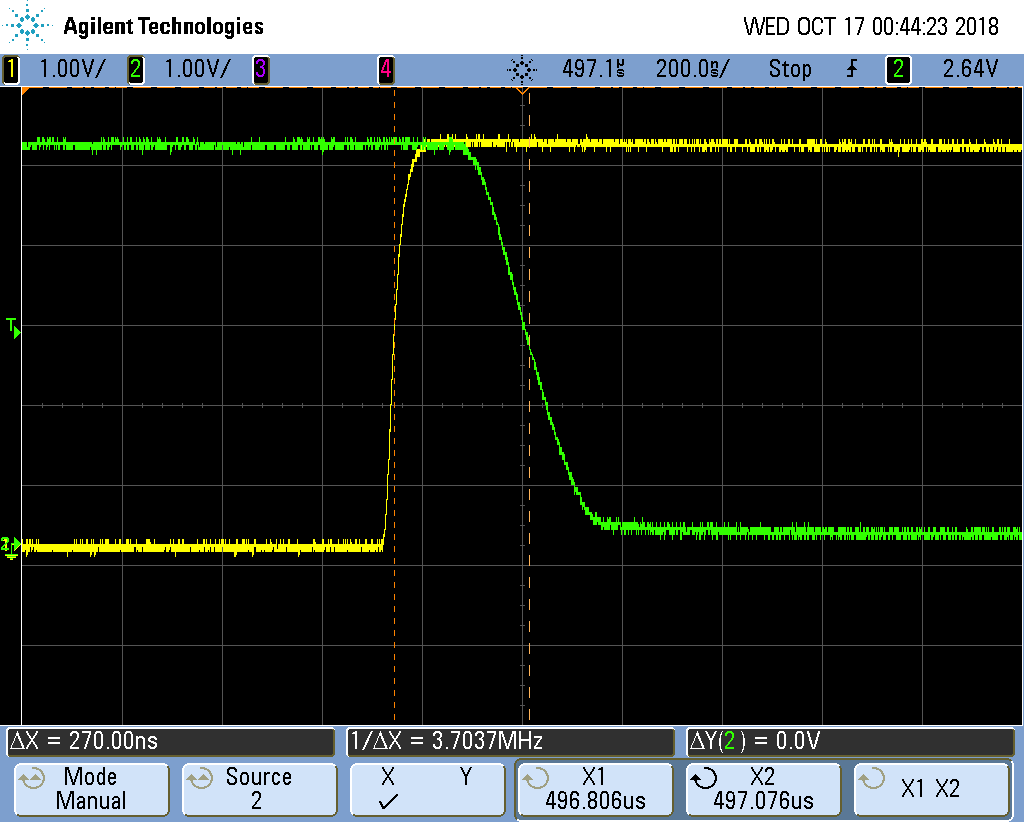
\includegraphics[width=0.4\textwidth]{ejercicio1/pHL-NPN}
    \caption{Medición Propagation Delay NPN: High to Low} %caption abajo
\end{figure}

\begin{figure}[H]
  \centering
    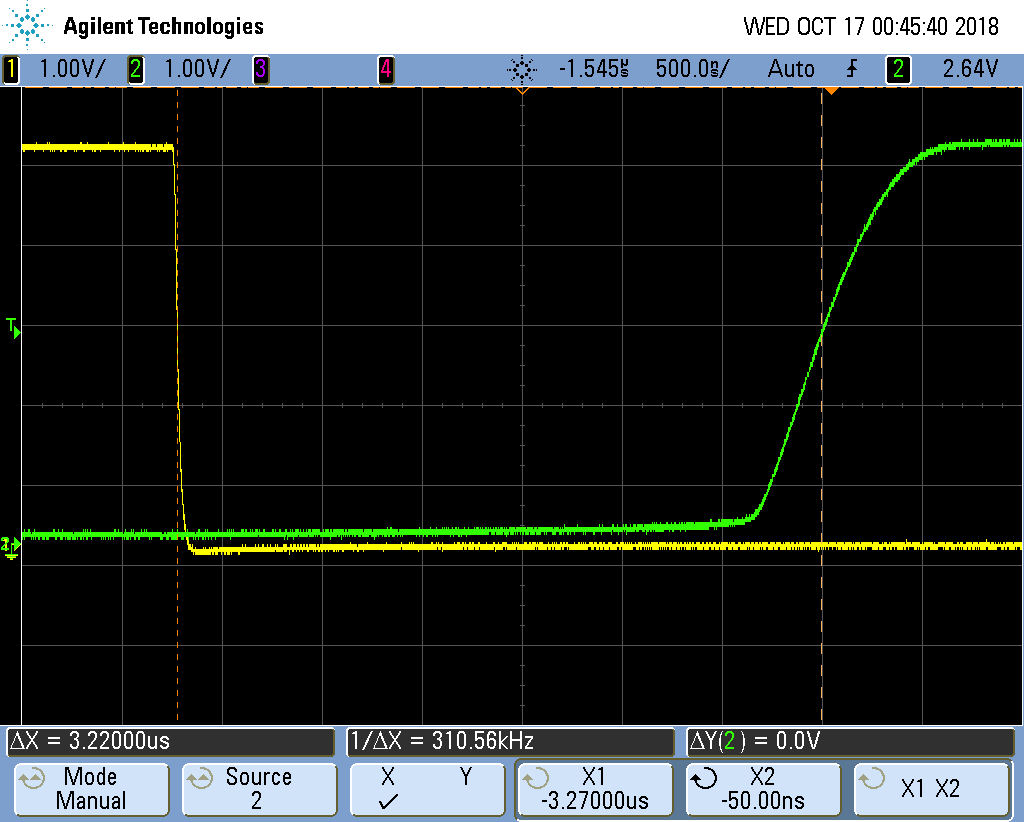
\includegraphics[width=0.4\textwidth]{ejercicio1/pLH-NPN}
    \caption{Medición Propagation Delay NPN: Low to High} %caption abajo
\end{figure}

\begin{figure}[H]
  \centering
    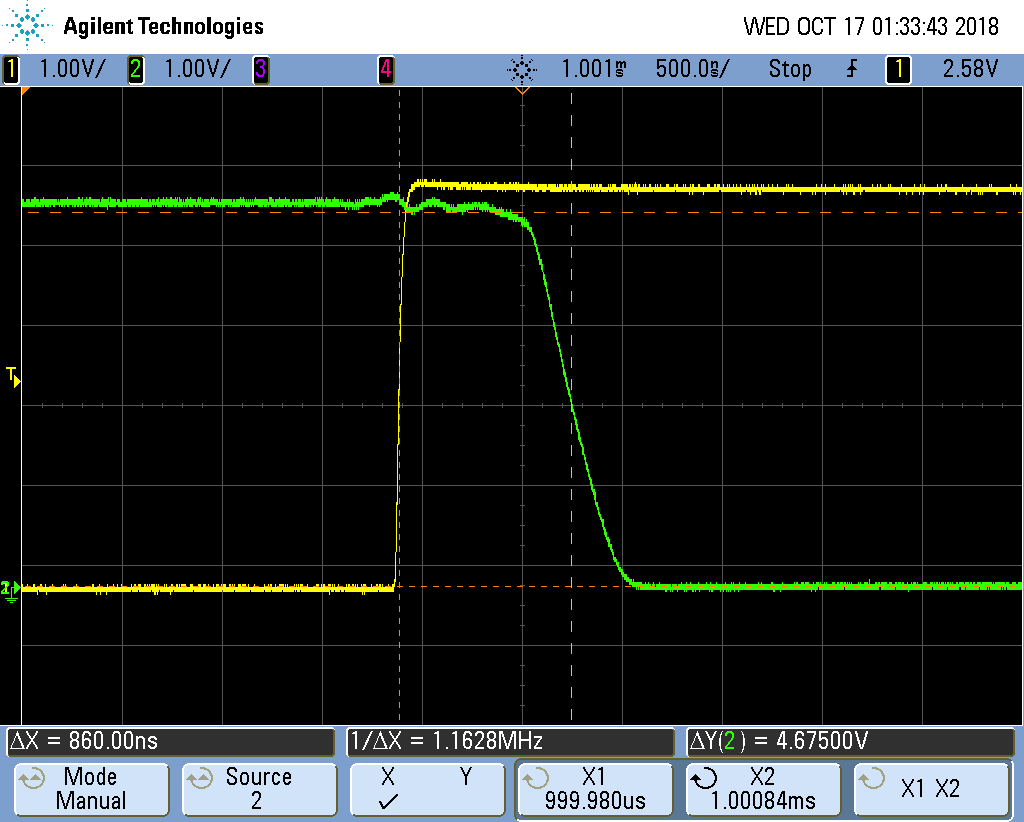
\includegraphics[width=0.4\textwidth]{ejercicio1/pHL-PNP}
    \caption{Medición Propagation Delay PNP: High to Low} %caption abajo
\end{figure}

\begin{figure}[H]
  \centering
    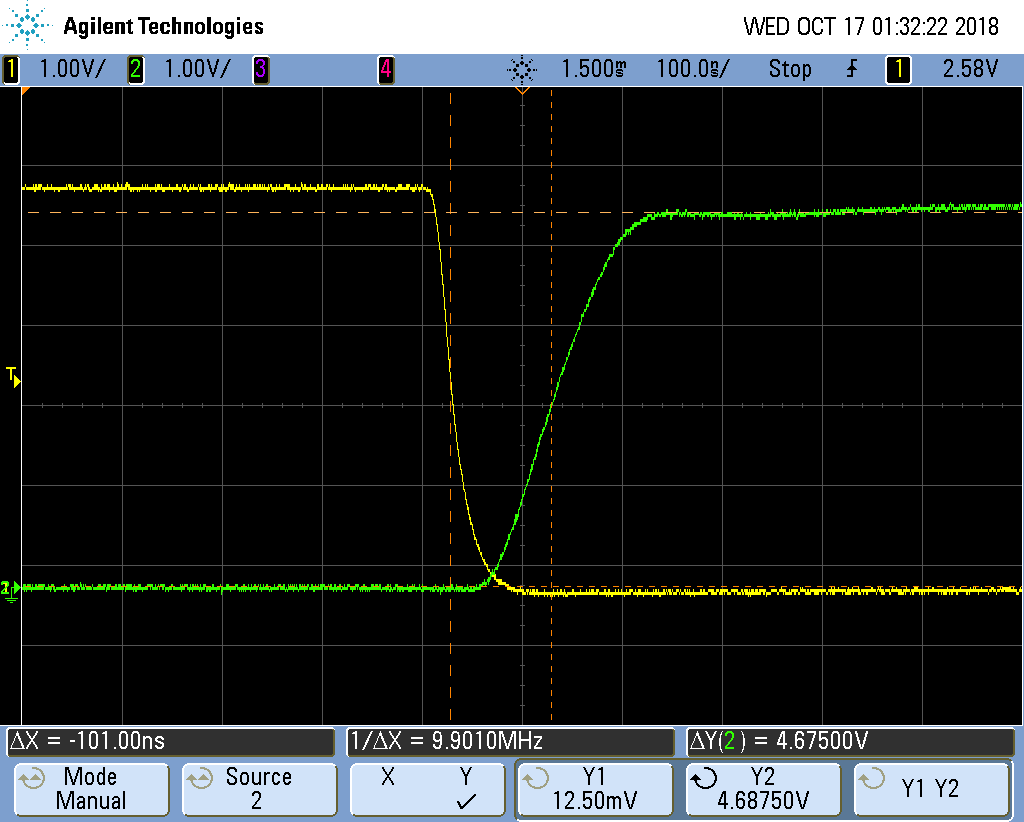
\includegraphics[width=0.4\textwidth]{ejercicio1/pLH-PNP}
    \caption{Medición Propagation Delay PNP: Low to High} %caption abajo
\end{figure}

\begin{figure}[H]% este es para caption arriba o abajo
  \centering
    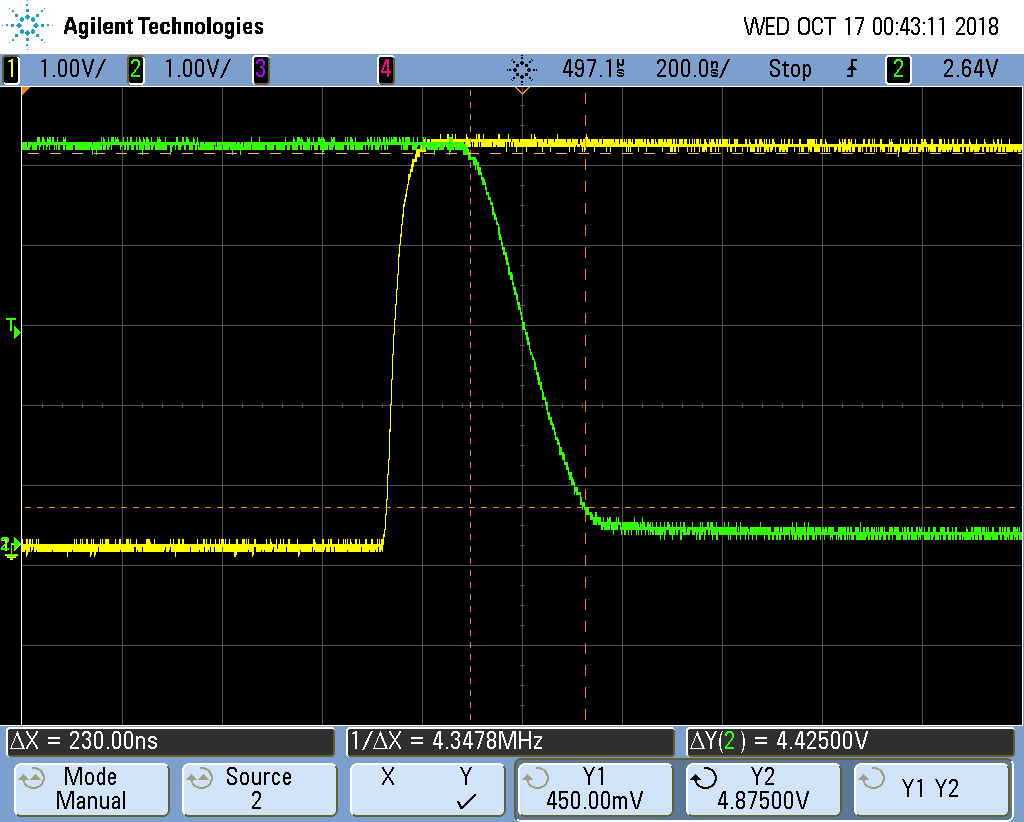
\includegraphics[width=0.4\textwidth]{ejercicio1/tHL-NPN}
    \caption{Medición Transition Time NPN: High to Low} %caption abajo
\end{figure}

\begin{figure}[H]
  \centering
    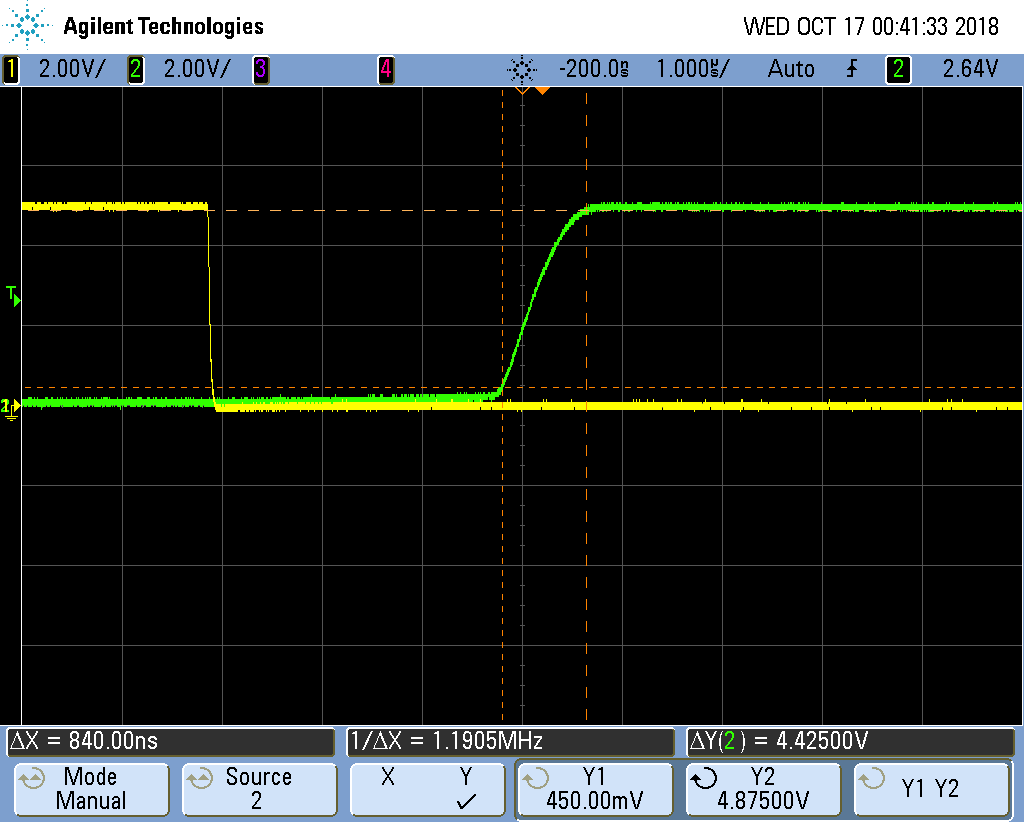
\includegraphics[width=0.4\textwidth]{ejercicio1/tLH-NPN}
    \caption{Medición Transition Time NPN: Low to High} %caption abajo
\end{figure}

\begin{figure}[H]
  \centering
    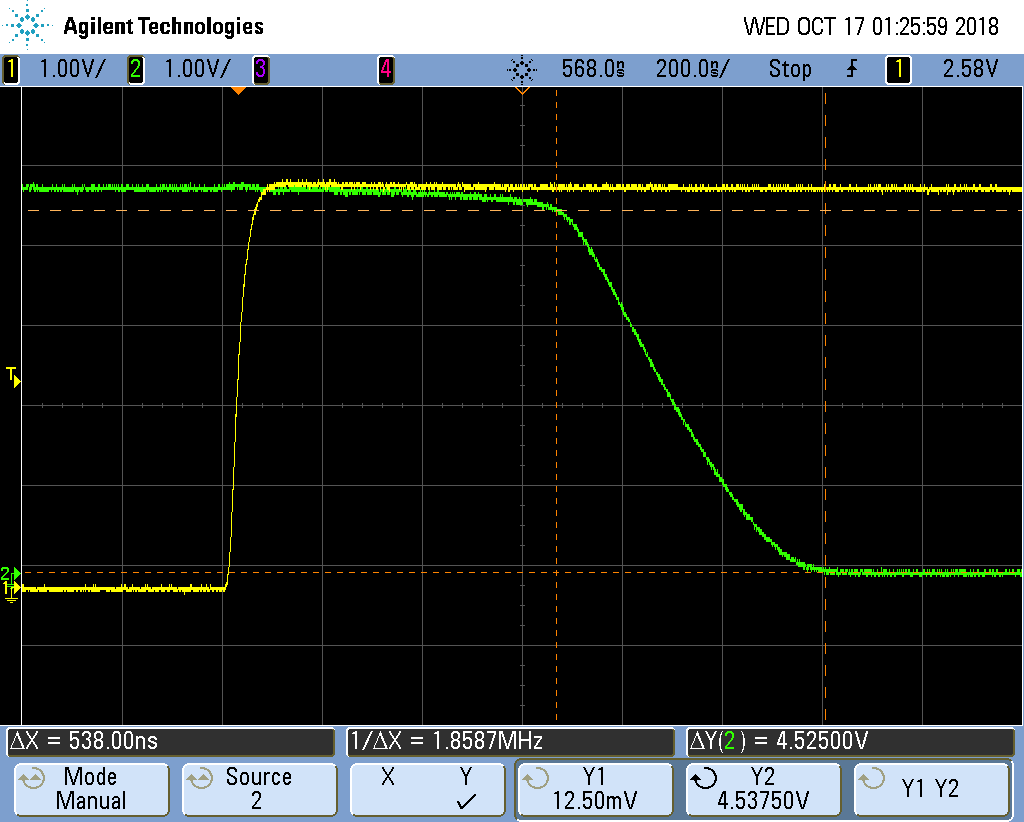
\includegraphics[width=0.4\textwidth]{ejercicio1/tHL-PNP}
    \caption{Medición Transition Time PNP: High to Low} %caption abajo
\end{figure}

\begin{figure}[H]
  \centering
    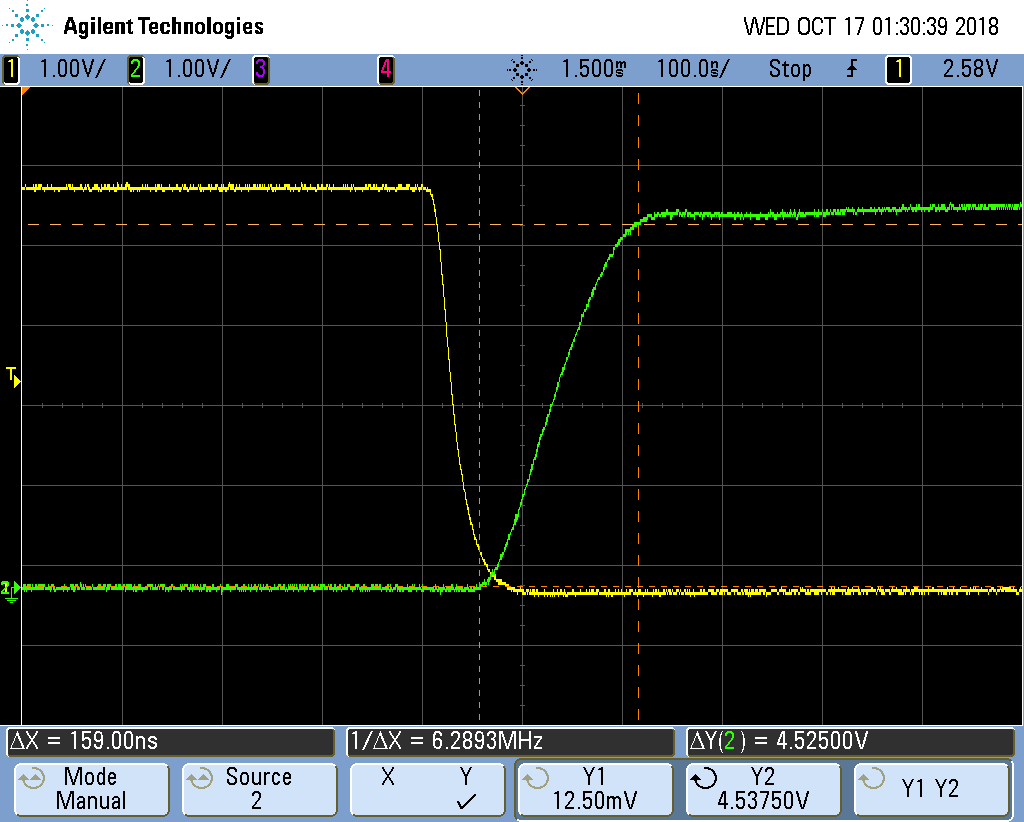
\includegraphics[width=0.4\textwidth]{ejercicio1/tLH-PNP}
    \caption{Medición Transition Time PNP: Low to High} %caption abajo
\end{figure}

\begin{figure}[H]
  \centering
    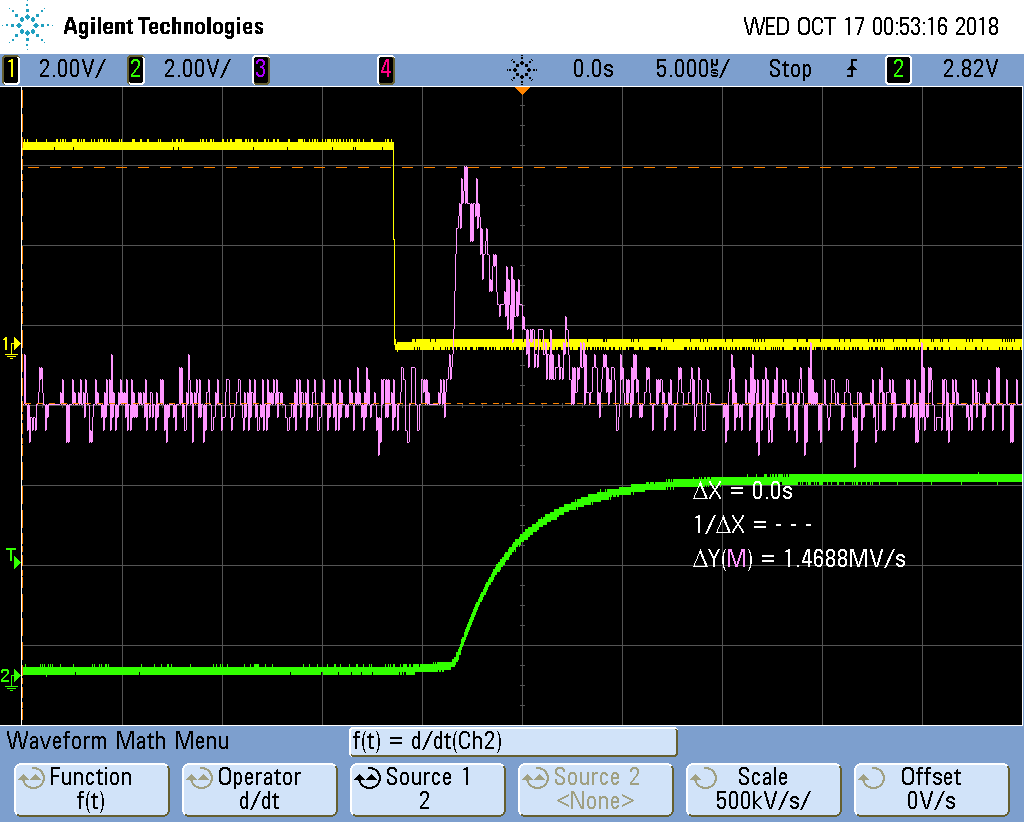
\includegraphics[width=0.4\textwidth]{ejercicio1/maxI-NPN}
    \caption{Medición máxima derivada de tensión en la salida NPN} %caption abajo
\end{figure}

\begin{figure}[H]
  \centering
    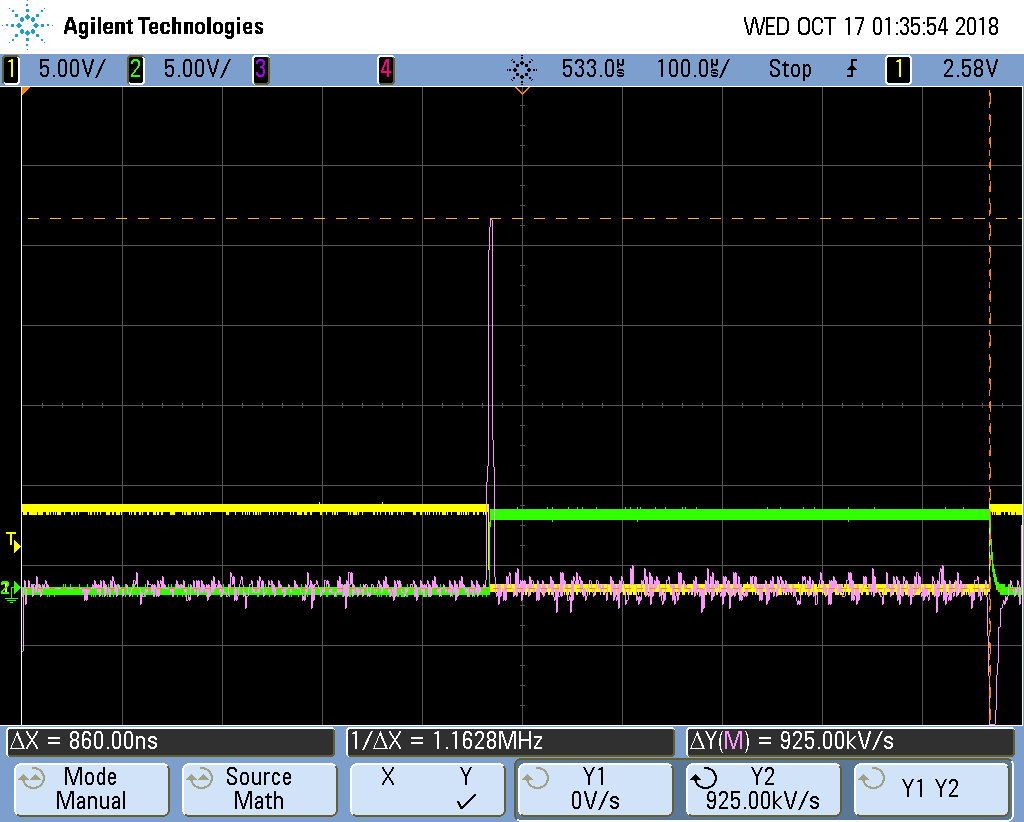
\includegraphics[width=0.4\textwidth]{ejercicio1/maxI-PNP}
    \caption{Medición máxima derivada de tensión en la salida PNP} %caption abajo
\end{figure}
\end{multicols}
